 \subsection{Camadas da Arquitetura Limpa}
        \par A Arquitetura Limpa tem por objetivo organizar o sistema em camadas concêntricas, ou seja, com dependências apontando para dentro, conforme a Regra da Dependência. As camadas incluem entidades, casos de uso, adaptadores de interface, frameworks e drivers, conectados por limites que garantem desacoplamento \cite{livro:martin:cleanarch}.
        
        \par Abaixo segue a explicação para cada um desses conceitos, que são a base para o entendimento da arquitetura limpa.

         \begin{figure}[H] % O [H] exige o uso do pacote float (veja abaixo)
            \centering
            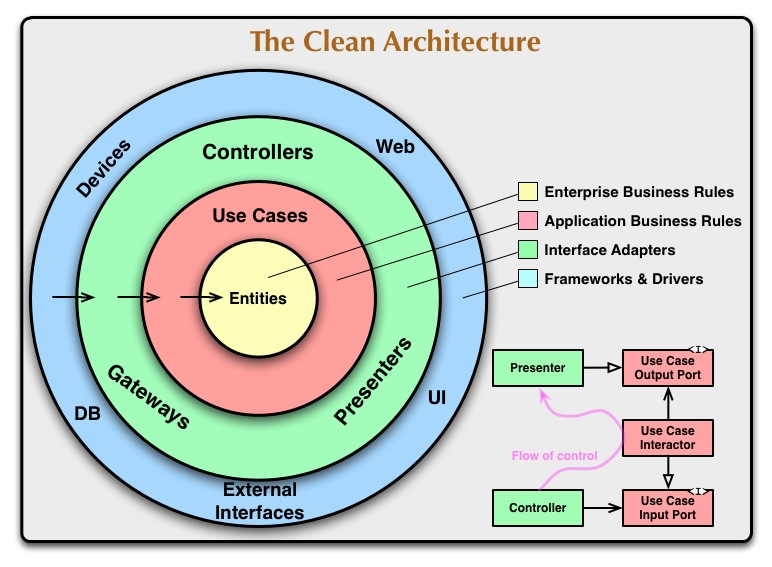
\includegraphics[width=0.8\textwidth]{figuras/clean_arch_1.jpg}
            \caption{A arquitetura limpa}
            \label{fig:figura_clean_arch_1}
            \newcommand{\minhafonteum}{Fonte: \cite{livro:martin:cleanarch}}
            \minhafonteum
        \end{figure}
        
        \subsubsection{Regra da Dependência}
        
            \par A Regra da Dependência é uma regra que visa estabelecer como as dependências devem se relacionar na arquitetura limpa. Ela define que dependências do código-fonte devem apontar para camadas internas, garantindo que nada em uma camada externa seja conhecido pelas camadas internas, incluindo funções, classes ou formatos de dados \cite{livro:martin:cleanarch}. 

            \par Nesse sentido, para realizar a implementação dessa regra é necessário o uso de interface abstratas, que isolam as camadas internas (entidades e casos de uso) dos detalher técnicos mais externo, como bancos de dados ou frameworks \cite{livro:martin:cleanarch}.

        \subsubsection{Entidades}
            \par As entidades são os componentes da arquitetura limpa responsáveis por encapsular as regras de negócio do software, sendo objetos ou coleções de dados e funções de tecnologias externas \cite{livro:martin:cleanarch, artigo:ferreira:2022, artigo:dantas:2021}. Elas fazem parte da camada central, que sofrera menos mudanças ao longo do tempo, e são a representação do domínio do sistemas. Além disso  as entidades garantem estabilidade, pois elas são desenvolvidas para não serem alteradas quando houver mudanças em interfaces ou bancos de dados \cite{artigo:dantas:2021, livro:martin:cleanarch}.
            
        \subsubsection{Casos de Uso}
            \par Os casos de uso são usados para realizar a implementação das regras de negócio específicas do software, orquestrando o fluxo de dados entre as entidades e outras camadas. Eles tem a característica de serem independentes de detalhes externos, com foco na intenção do negócio e também permitem que o desenvolvimento do software seja incremental e que os testes possam ser feitos de maneira isolada. \cite{artigo:ferreira:2022, livro:martin:cleanarch}
            
        \subsubsection{Adaptadores de Interface}

            \par Os adaptadores de interface são responsáveis por converter dados de formatos internos (usado por casos de uso e entidades) e externos (como bancos de dados e APIs), eles servem para isolar os detalhes técnicos da lógica do negócio da aplicação, também são úteis para facilitar a substituição de tecnologias externas sem afetar as camadas mais internas do software \cite{livro:martin:cleanarch}. 
            
        \subsubsection{Frameworks e Drivers}

            \par Os frameworks e drives representam as ferramentas e tecnologias externas, como bancos de dados, frameworks e dispositivos que fazem entrada ou saída de dados, considerado detalhes de implementação que podem mudar ao longo do tempo de desenvolvimento dos projetos \cite{livro:martin:cleanarch}.